\section{Case Study: Shopping Carts}
\label{sec:carts}

\begin{figure}
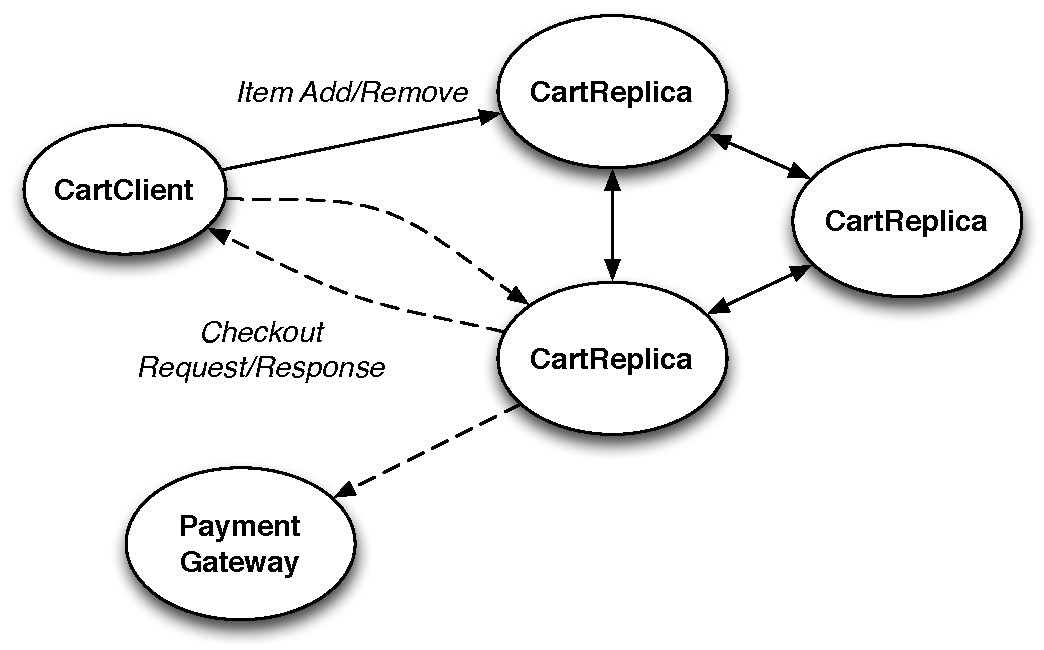
\includegraphics[width=\linewidth]{fig/cart_arch.pdf}
\label{fig:cart-system}
\caption{Architecture of a simple shopping cart system.}
\end{figure}

In this section, we consider a simple e-commerce system in which clients
interact with a shopping cart service, adding and removing items over the course
of their browsing session (Figure~\ref{fig:cart-system}). Eventually, a client
submits a ``checkout'' operation, at which point the cumulative effect of their
shopping session should be summarized and returned to the client. In a more
complete system, the result of the checkout operation might be presented to the
client for confirmation or submitted to a payment processor to complete the
e-commerce transaction. This case study is based on the cart system from Alvaro
et al.~\cite{Alvaro2011}, which was in turn inspired by the discussion of
replicated shopping carts in the Dynamo paper~\cite{DeCandia2007}.

Alvaro et al.\ consider two different cart designs: a ``disorderly'' version in
which the cart state is represented as a set (allowing monotonic accumulation of
add/remove operations) and a ``destructive'' version in which the cart state is
managed by a key-value store, which requires a non-monotonic update on each cart
action. In both designs, Alvaro et al.\ argue that the checkout operation must
be non-monotonic, because it requires aggregating over all previous operations
applied to the cart. Non-monotonic operations are potentially expensive because
they might require coordination to produce consistent results.

In this section, we detail two modifications to the cart design that can be
implemented using lattices. First, we discuss how the ``destructive'' design can
be made monotonic.

\subsection{Multiset Lattice}

\subsection{Monotonic Checkout}
